% Created 2014-06-26 ���� 15:54
\documentclass[11pt]{article}
\usepackage[utf8]{inputenc}
\usepackage[T1]{fontenc}
\usepackage{fixltx2e}
\usepackage{graphicx}
\usepackage{longtable}
\usepackage{float}
\usepackage{wrapfig}
\usepackage{soul}
\usepackage{textcomp}
\usepackage{marvosym}
\usepackage{wasysym}
\usepackage{latexsym}
\usepackage{amssymb}
\usepackage{hyperref}
\tolerance=1000
\providecommand{\alert}[1]{\textbf{#1}}

\title{make things easier and more maintainable}
\author{}
\date{\today}
\hypersetup{
  pdfkeywords={},
  pdfsubject={},
  pdfcreator={Emacs Org-mode version 7.9.3f}}

\begin{document}

\maketitle

\setcounter{tocdepth}{3}
\tableofcontents
\vspace*{1cm}

\section{introduce}
\label{sec-1}
\subsection{how we use javascript as before}
\label{sec-1-1}
\subsubsection{use.as.normal.function.js}
\label{sec-1-1-1}



\begin{verbatim}

<script src="~/Scripts/Jquery/jquery-1.8.0.min.js"></script>

$(function () {
  // do something after dom ready
});
\end{verbatim}
\begin{itemize}

\item drawback
\label{sec-1-1-1-1}%
\begin{itemize}
\item 依赖不明显
\item 重复加载
\item 污染全局变量
\end{itemize}


\item what can we do ? use as module !
\label{sec-1-1-1-2}%
\begin{itemize}
\item Why
\begin{itemize}
\item 解耦,职责单一,高内聚\ldots{}
\item 模块本身可控,更容易解决依赖(新增,删除..)
\item 平滑过渡
\end{itemize}
\item How
      原生的javascript本身没有这方面的设计,只能借助框架||规范
\begin{itemize}
\item cmd
\item amd
\end{itemize}
\end{itemize}

\end{itemize} % ends low level
\subsection{CommonJS or AMD}
\label{sec-1-2}

\begin{itemize}
\item 都是为了模块化开发
\item AMD A means Asynchronous
     loaded as they are needed
     更适用于 cs (in-borwser)开发
\item CommonJs
     loading all modules up front
     更适用于 server-side (node.js..)
\item 为了推广,其实双方都可以同步也可以异步.侧重点不同.
\end{itemize}
\subsubsection{use.as.module.js}
\label{sec-1-2-1}



\begin{verbatim}
/*
  commonjs
*/
// package/lib is a dependency we require
var lib = require( "package/lib" );

// behavior for our module
function foo(){
    lib.log( "hello world!" );
}

// export (expose) foo to other modules as foobar
exports.foobar = foo;

/*
  AMD
*/
// package/lib is a dependency we require
define(["package/lib"], function (lib) {

    // behavior for our module
    function foo() {
        lib.log( "hello world!" );
    }

    // export (expose) foo to other modules as foobar
    return {
        foobar: foo
    }
});

require(["package/myModule"], function(myModule) {
    myModule.foobar();
});
\end{verbatim}
\section{how we use amd in our proj}
\label{sec-2}

  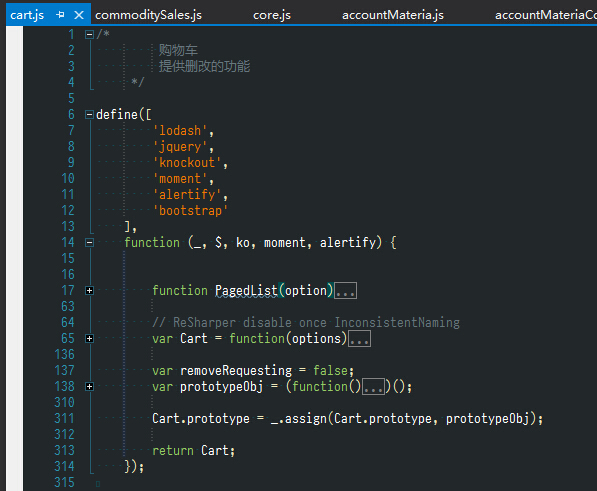
\includegraphics[width=.9\linewidth]{requirejs.cart.jpg}
\section{what else can we do ?}
\label{sec-3}

  use it whth knockout.js (js MVVM Framework)\\
  see a sample\\
  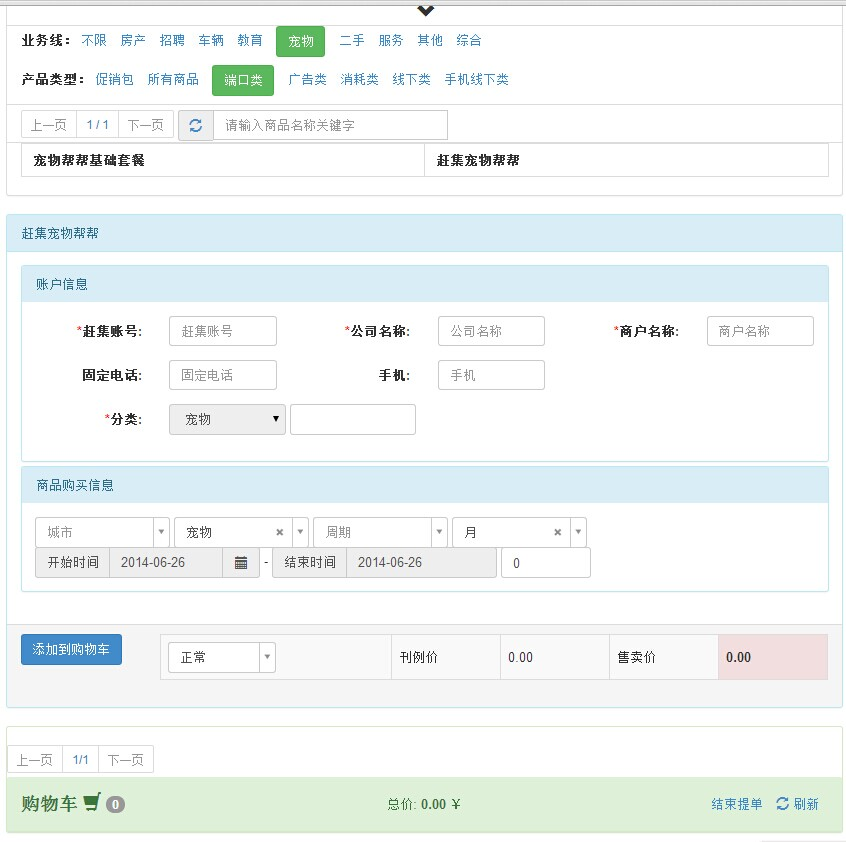
\includegraphics[width=.9\linewidth]{shopping.view.jpg}

\begin{itemize}
\item 模块化页面
    分离为各个小型 widget
\begin{itemize}
\item 便于一定程度的重用,便于管理维护
\item 问题: 如何进行widget间的交互?
\item 通过事件通知机制,避免直接相互依赖,相互耦合
\end{itemize}
\item 既然模块化了js widget,如何实现 view 和 js 分离
\begin{itemize}
\item 分离以后,数据通讯怎么做? no razor !
\item 服务端的数据 (ajax request url\ldots{}) 如何传递给 js 文件?
\item 全局变量存储 js 变量,进行传递
\end{itemize}
\item code smell
\begin{itemize}
\item 尽可能少的用 razor 对 html 结构进行控制.
\item 尽可能使用js模板引擎进行控制,使前端更前端,更能less is more的高效处理
\item 尽可能少的使用 \$ 对dom进行动态变更,使用 mvvm 的双向绑定进行控制
\item 尽可能在html中使用声明式编程,在后端用程序赋予每个声明具体的意义(因为html设计的本意就不是为了展现动态页面.html5?)
\end{itemize}
\end{itemize}

  see a demo => \href{http://uniorder.test.corp.ganji.com/shop/apply?ContractId=22362&contractSourceType=1}{http://uniorder.test.corp.ganji.com/shop/apply?ContractId=22362\&contractSourceType=1}

\end{document}
